\documentclass{article}
\usepackage{wrapfig}
\usepackage{rotating}
\usepackage{graphicx}
\usepackage{mathtools}
\usepackage{multicol}
\usepackage[backend=biber, bibencoding=utf8]{biblatex}
\usepackage[margin=1.2in]{geometry}
\usepackage{booktabs}
\usepackage{enumerate}
\usepackage{caption}
\addbibresource{oirefs.bib}


\title{Facial Analysis of Patient Affected by Osteogenesis
Imperfecta Using Computer Vision}


\author{
Rousseau, Maxime\\
\texttt{maxime.rousseau2@mail.mcgill.ca}
\and
Retrouvey, Jean-Marc\\
\texttt{@mcgill.ca}
\and
Rauch, Frank\\
\texttt{@mcgill.ca}
\and
Vargas, Javier\\
\texttt{@mcgill.ca}
}

\begin{document}

\maketitle
\begin{multicols}{2}


\section{Abstract}

Individuals affected by Osteogenesis Imperfecta (OI), an autosomal
dominant genetic disease mainly affecting the COL1A1/A2 genes, have been
reported to demonstrate characteristic facial manifestations of the
disease. This study uses computer vision and statistical shape analysis
to compare the antero-posterior photographs of individuals affected by
OI to photographs from a normocephalic control group. Intergroup
analysis was also conducted. Facial analysis of subjects affected by
Osteogenesis Imperfecta types I, III and IV shows that the facial index
is significantly different when compared to controls. Results also point
out strong similarities between types I and IV in terms of severity of
the facial manifestations and morphology. Previous qualitative
literature reports of facial manifestations of OI were validated by our
results. Comparison to a baseline shape allowed to pinpoint a typical
facial pattern presented by OI individuals. Furthermore, successful
classification of patient was performed used logistic regression models.

\section{Introduction}

Osteogenesis imperfecta is a rare bone disease of genetic etiology. It
is autosomal dominant in most cases and mainly affects the COL1A1/A2
genes related to the production of collagen. Other mutations have also
been reported (Eimar et al. 2016). The range of phenotypes and severity
are wide. Bone fragility is the main issue amongst subjects affected.
Subjects often present with a much higher rate of long bone fractures
and growth issues (Rauch and Glorieux 2004). Four main types of OI have
been described (Chang, Lin, and Hsu 2007) and are based on phenotypes.
In order of increasing severity, they are types I, IV, III and II (II
being lethal at birth). There is no cure for OI and treatment usually
involves the use of IV bisphosphonates (Drake, Clarke, and Khosla 2008).
These genetic alterations have craniofacial implications for individuals
affected by OI. Only qualitative reports currently address the facial
morphology of these patients in the literature. The goal of this study
is to explore the facial characteristics of OI types I, III and IV
subjects~in a quantitative manner and expand on the observations made in
the literature. The method leverages computer vision and machine
learning to accelerate, standardize and broaden the data gathering
effort. A morphological approach relying on a statistical shape
methodology was used to conduct our analysis (Ian L. Dryden 2012). We
decided that this would be the most accurate method to compare the
facial shapes obtained by image processing as it allows for rotation and
resizing to summarize a group into a mean shape. Using landmarks also
allows us to compute diverse metrics to isolate the differences from an
anatomical perspective. The null hypothesis is that there are no
statistically significant differences in the facial morphology of
subjects affected by different types of OI when compared to
normocephalic patients. The authors propose models based on facial
landmark which could be considered as a clinical aid to classification
and diagnosis to Osteogenesis Imperfecta.

\section{Study Design}

A case-control study was conducted on a total of 306 (M:145/F:161)
patients. The Individuals affected by OI where part of the BBDC 7701
study conducted at Shriners Hospital in Montreal, Canada. These patients
were grouped according to their OI classification. The first group
consisted of 88 (42/46) OI type I subjects. A second group was composed
of 28 (9/19) OI type III subjects. The third group consisted of 57
(26/31) OI type IV subjects. The control group consisted of 133 (68/65)
patients (Figure 1). Population testing for sex (Chi-Squared) and age
(ANOVA) showed no statistically significant difference between the
groups (Table 1). The selection criteria for the control group was to
present a facial index 0.80 which is considered as the ideal facial
proportions between height and width of the face (Franco et al. 2013).
The measurement is a ratio of face height by the bizygomatic width. This
index was preferred for the control group as it is deemed preferable to
have a uniform control group to identify the facial characteristics of
OI subjects. Having a static baseline would allow us to better isolate
the discrepancies presented by patients affected by OI.


\begin{center}
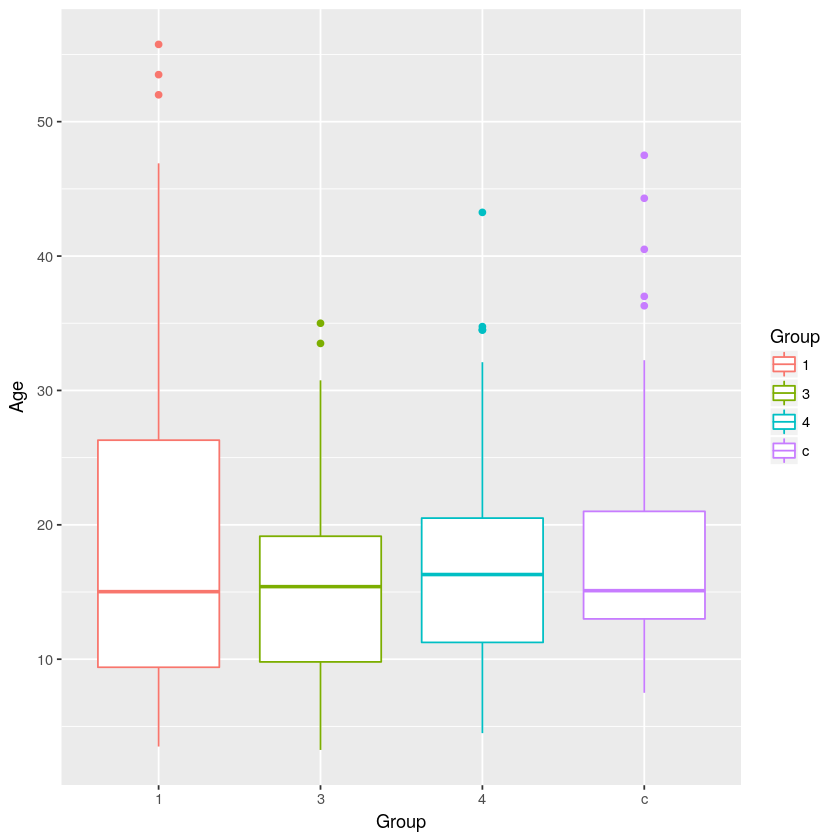
\includegraphics[width=\linewidth]{figures/sample.png}
\captionof{figure}{Population sample ages}
\end{center}

\section{Materials and Methods}

Antero-posterior photographs of the subjects' faces were used for this
analysis. These pictures where all taken by the same operator using a
Canon D 70 Dental Eye camera following the McGill University photography
protocol. Pictures that did not meet the requirements for a proper
extra-oral orthodontic photograph were excluded from the study. The
python and R notebooks used in this study were published on GitHub. This
study makes use of the OpenCV (Itseez 2017) open source computer vision
library, the Dlib library and a publicly available facial annotation
tool (Sagonas et al. 2013). The machine learning models were written
with the Scikit Learn library. This program detected the patients faces
through a process called a Haar cascade (Viola and Jones 2001). After
having fitted the face to a rectangle, 68 landmarks were automatically
identified on each facial photograph (Figure 1). The algorithm placing
the landmarks was pre-trained on 300 sample faces. X, Y coordinates from
these landmarks were stored in matrices for use in our statistical
analysis.

\begin{center}
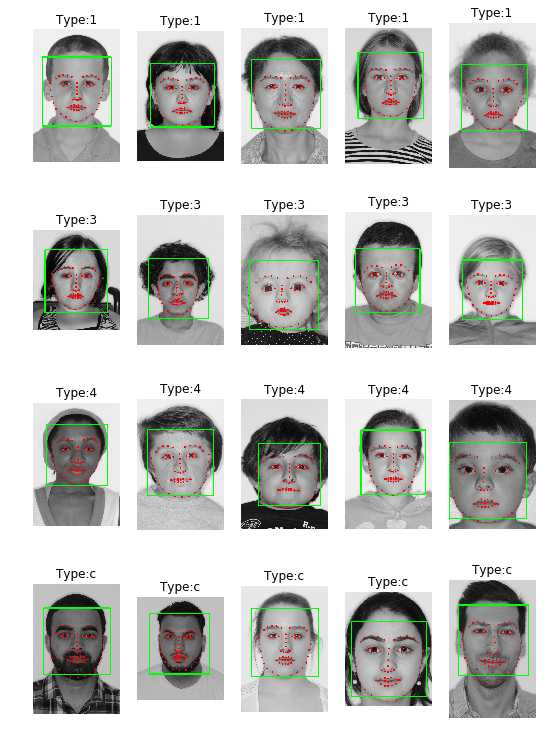
\includegraphics[width=\linewidth]{figures/processing.png}
\captionof{figure}{Face Detection and Landmark Placement}
\end{center}

To be able to compare the landmarks further manipulations were done
using the R statistical programming language as well as the Shapes
package (Dryden 2017). The landmark data of each groups was then
processed using Generalized Procrustes Analysis (GPA). This algorithm
scaled and rotated the shapes within a group for optimal fit then
computed the mean shape for the group. A new group landmark dataset was
saved using the rotated and scaled landmark coordinates. This dataset
was then used to compute all our metrics for statistical analysis and
train classifiers.


The mean shapes were used for the comparison of the affected groups to
the control group. An intergroup analysis was also conducted. These
comparisons were computed with Goodall's F-Test for statistical
significance. Using the mean shape of the control group as a baseline,
the distance of each landmark from the baseline coordinates were also
computed for each patient. This distance was calculated using Euclidean
geometry to get an absolute value. The results were compiled as mean
distances per landmark for each group to detect the differences in the
morphologies of the OI types. The population mean value was set using
the control group. Three facial ratios and the lower face height (LFH)
of each patient were also computed for each patient using the same set
of landmarks coordinates (Figure 3). Z-scores were computed for each
metric. The groups were tested using ANOVA with Bonferroni post-hoc
tests (table 1).

\begin{center}
  \begin{enumerate}[(a)]
\item \[MED=\dfrac{\sum_{n=1}^{68} \sqrt{(b_i^x-l_i^x)^2+(b_i^y-l_i^y)^2}}{68}\]
\item \[R_1=(l_{46}-l_{37})/(l_{17}-l_1)\]
\item \[R_2=(l_{13}-l_5)/(l_{17}-l_1)\]
\item \[R_3=(l_{17}-l_1)/(l_{28}-l_9)\]
\item \[LFH=(l_{34}-l_{9})/(l_{28}-l_{9})\]
\end{enumerate}
\captionof{figure}{Equations of the measurements taken from the samples for our statistical analysis}
\end{center}

\begin{center}
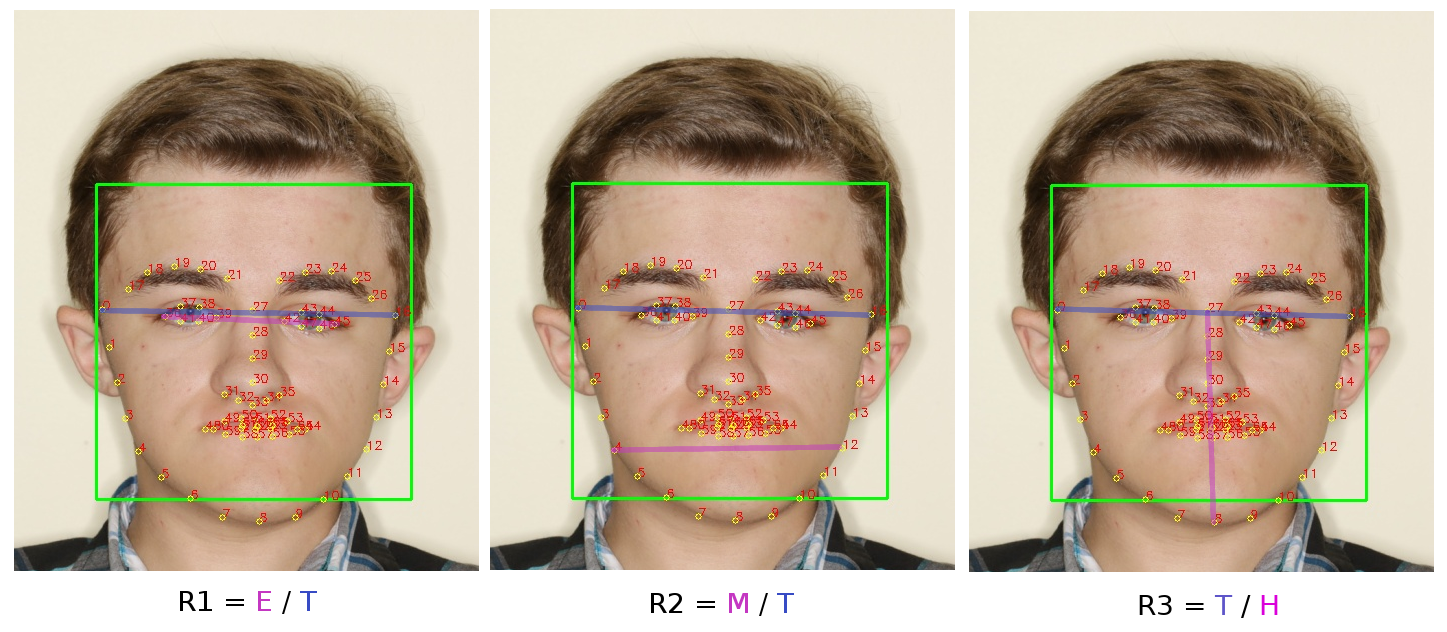
\includegraphics[width=\linewidth]{figures/ratios.png}
\captionof{figure}{Facial Ratios Used for Facial Analysis}
\end{center}

Three different classifiers were trained, all of which had the same
architecture. The input layer consisted of 138 features. 68 x and y
coordinates as well as the age and sex of the patient. Principal
component analysis was used to reduce the dimension to 30 features which
were then passed through a logistic regression (Figure 4). The
train/test set were created from an 80/20 split of the dataset. Two
binary classifiers were trained as well as one multiclass classifier.
The first binary classifier was used to classify controls and OI type I
patient as these are sometimes hard to distinguish clinically. The
second one, was had to detect whether the patient was affected by OI
(all types included). The multiclass model had to detect whether the
patient was a control, OI type I/IV or OI type III.


\begin{center}
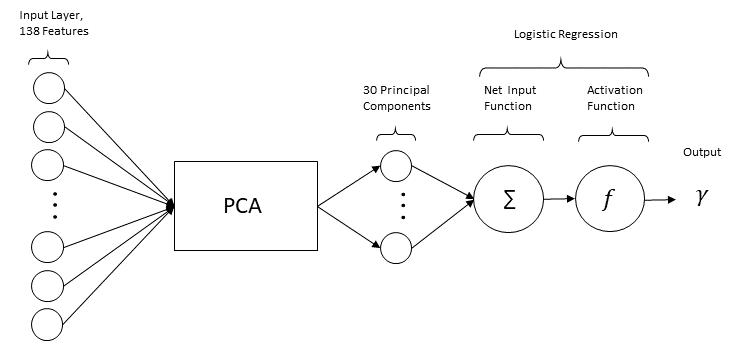
\includegraphics[width=\linewidth]{figures/regression.png}
\captionof{figure}{Schematic Representation of Classifiers}
\end{center}

\section{Results}

The p-values obtained from the mean shape comparison of the groups were
all statistically significant except for the comparison between subjects
affected by type I OI to those affected by type IV. The results of our
other analyses are summarized in Table 1.

\begin{table*}
\begin{center}
\resizebox{\linewidth}{!}{
\begin{tabular}{lrrrrr}
\toprule[\heavyrulewidth]\toprule[\heavyrulewidth]
 & Control & OI Type I & OI Type III & OI Type IV & P-Value\\
\midrule
	N (M/F) & $133 (68/65)$ & $88 (42/46)$ & $28 (9/19)$ & $57 (26/31)$ &
	P(Chi-Squared) = $0.32$\\
	Age (years) & $17.7 (7.7)$ & $19.7 (14)$ & $15.4 (8.4)$ & $17.1 (8.4)$ & P(ANOVA) =
	$0.19$\\
	MED & $NA$ & $0.0075^{bc} (0.005)$ & $0.0106^{c} (0.008)$ & $0.0081 (0.006)$ &
	P(ANOVA)  $<0.05$\\
	MED Z-Score & $NA$ & $-0.122^{bc} (0.907)$ & $0.439^{c} (1.156)$ & $-0.027
	(0.995)$ & P(ANOVA) $<0.05$\\
	Ratio 1 & $0.612^{a} (0.026)$ & $0.595 (0.026)$ & $0.604 (0.036)$ & $0.602
	(0.031)$ & P(ANOVA) $<0.05$\\
	Ratio 1 Z-Score & $0.246^{a} (0.901)$ & $-0.323 (0.926)$ & $0.008 (1.242)$ &
	$-0.080 (1.069)$ & P(ANOVA) $<0.05$\\
	Ratio 2 & $0.799^{a} (0.027)$ & $0.784 (0.038)$ & $0.774 (0.030)$ & $0.791
	(0.031)$ & P(ANOVA) $<0.05$\\
	Ratio 2 Z-Score & $0.247^{a} (0.839)$ & $-0.215 (1.175)$ & $-0.537 (0.912)$ &
	$0.021 (0.944)$ & P(ANOVA) $<0.05$\\
	Ratio 3 & $1.26^{abc} (0.075)$ & $1.33^{b} (0.106)$ & $1.40^{c} (0.124)$ &
	$1.33 (0.097)$ & P(ANOVA) $<0.05$\\
	Ratio 3 Z-Score & $-0.444^{abc} (0.726)$ & $0.264^{b} (1.02)$ & $0.909^{c}
	(1.191)$ & $0.181 (0.938)$ & P(ANOVA) $<0.05$\\
	LFH & $0.569 (0.022)$ & $0.571 (0.027)$ & $0.562 (0.035)$ & $0.567 (0.026)$ &
	P(ANOVA) = $0.47$ \\
	LFH Z-Score & $0.0185 (0.871)$ & $0.0818 (1.02)$ & $-0.253 (1.407)$ &
	$-0.045 (1.021)$ & P(ANOVA) = $0.47$\\
\bottomrule[\heavyrulewidth]
\end{tabular}}
\captionof{table}{Results from the Measurements and Statistical
Testing. a: $p<0.05$ in comparison to OI-I b: $p<0.05$ in comparison to OI-III
c: $p<0.05$ in comparison to OI-IV}
\end{center}
\end{table*}

The accuracy metrics for the different models are summarized in table 2.
We can see the confusion matrices of the models in figure 5.

\begin{center}
\resizebox{\linewidth}{!}{
\begin{tabular}{lrrrrr}
\toprule[\heavyrulewidth]\toprule[\heavyrulewidth]
	Model & Class & Precision & Recall & F1-Score & Support\\
\midrule
	OIM0 & Control & 1.00 & 1.00 & 1.00 & 27 \\
		 & OI Type 1 + 4 & 0.97 & 1.00 & 0.98 & 29 \\
		 & OI Type 3 & 1.00 & 0.80 & 0.89 & 5 \\
		 & Total & 0.98 & 0.98 & 0.98 & 61 \\
\midrule
	OIB0 & Control & 1.00 & 1.00 & 1.00 & 26 \\
		 & OI Type 1 & 1.00 & 1.00 & 1.00 & 18 \\
		 & Total & 1.00 & 1.00 & 1.00 & 44 \\
\midrule
	OIB1 & Control & 1.00 & 1.00 & 1.00 & 25 \\
		 & OI Subject & 1.00 & 1.00 & 1.00 & 36 \\
		 & Total & 1.00 & 1.00 & 1.00 & 61 \\
\bottomrule[\heavyrulewidth]
\end{tabular}}
\captionof{table}{Accuracy Metrics from the Classifiers Test Set}
\end{center}

\section{Discussion}

Considering the body of results obtained, the null hypothesis is
rejects. This confirms previous literature reports of a different facial
morphology for the patients affected by OI. Mean shape testing seems to
be more robust at detecting morphological differences in between the
group though it provides us with less insight. However, by visualizing
the results for the MED (Figure 6) we can see that the landmark situated
at the temples (1 and 17) and the lateral edges of the eyes (27 and 46)
account for much of the discrepancies that are observed. This seems to
be related to the triangular facial morphology described in previous
articles. CBCT imaging had also revealed prominent temporal bones in
patients affected by OI. When looking at the other metrics computed to
assess the facial characteristics of the patients we see that the ones
involving the bitemporal width will show statistically significant
results. On the other hand, the LFH measurement which only takes the
vertical aspect of the face into account was the only metric that showed
no intergroup differences. Also, similarly to the mean shape test, the
MED metric seem to be more reliable when comparing the facial morphology
of the subjects than any other single measurement taken. It is also
intuitive that a method which encompasses more landmarks enables for a
more accurate analysis. The ability to train successful classifiers
using landmarks and general patient data as input features also opens
the door to potential diagnostics aids. Given that OI is a rare disease
the main limitation to the sophistication of the models is the size of
the dataset. However, simple models can still be an effective diagnostic
aid for clinicians lacking an expertise in rare genetic bone disease.

% \begin{center}
% 
% 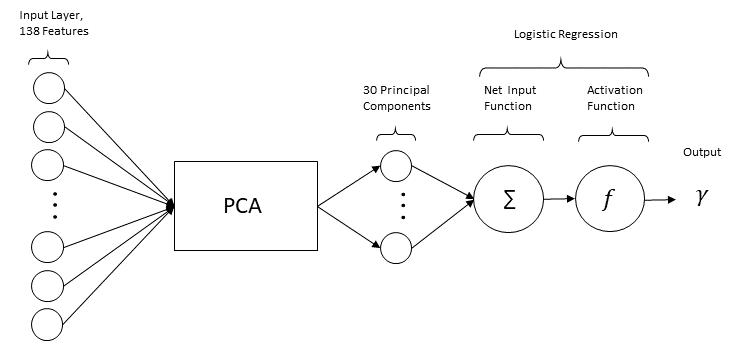
\includegraphics[width=\linewidth]{figures/regression.png}
% \captionof{figure}{Confusion Matrices of the Classifiers}}
% 
% \end{center}

\section{Conclusions}

Our results confirm the previous reports in the literature reporting
specific facial characteristics in subjects affected by Osteogenesis
Imperfecta. Our analysis also suggests that these manifestations are
present to varying degrees depending on the classification of the
disease and that type III group is the more severely affected. The
different facial analysis ran on these patients seem to point to
deformities at the level of the temples jaw and facial height relative
to the patient's general morphology. The findings of this study indicate
potential issues in the phenotypic classification initially put forth by
Sillence. The strong similarities between the patient from the type I
and type IV groups challenge our current understanding of the facial
manifestations of the disease. The findings of this study give us new
insight as to where to look for discrepancies with normal patients when
it comes to the facial characteristics of individuals affected by
Osteogenesis Imperfecta. The next step will be to determine the extent
of these differences and devise method to identify the severity of the
disease through automated facial recognition software.

\section{References}

Chang, P. C., S. Y. Lin, and K. H. Hsu. 2007. 'The craniofacial
characteristics of osteogenesis imperfecta patients', \emph{European
Journal of Orthodontics}, 29: 232-7.

Drake, M. T., B. L. Clarke, and S. Khosla. 2008. 'Bisphosphonates:
mechanism of action and role in clinical practice', \emph{Mayo Clinic
Proceedings}, 83: 1032-45.

Dryden, I. L. 2017. "shapes package." In. Vienna, Austria: R Foundation
for Statistical Computing.

Eimar, H., F. Tamimi, J. M. Retrouvey, F. Rauch, J. E. Aubin, and M. D.
McKee. 2016. 'Craniofacial and Dental Defects in the Col1a1Jrt/+ Mouse
Model of Osteogenesis Imperfecta', \emph{Journal of Dental Research},
95: 761-8.

Franco, F. C., T. M. de Araujo, C. J. Vogel, and C. C. Quintao. 2013.
'Brachycephalic, dolichocephalic and mesocephalic: Is it appropriate to
describe the face using skull patterns?', \emph{Dental Press J Orthod},
18: 159-63.

Ian L. Dryden, Kanti V. Mardia. 2012. \emph{Statistical Shape Analysis:
With Applications in R} (John Wiley \textbackslash{}\& Sons).

Itseez. 2017. "Open Source Computer Vision Library." In.:
\textbackslash{}url\{\url{https://github.com/itseez/opencv}\}.

Rauch, F., and F. H. Glorieux. 2004. 'Osteogenesis imperfecta',
\emph{Lancet}, 363: 1377-85.

Sagonas, C., G. Tzimiropoulos, S. Zafeiriou, and M. Pantic. 2013. 'A
Semi-automatic Methodology for Facial Landmark Annotation': 896-903.

Viola, P., and M. Jones. 2001. "Rapid object detection using a boosted
cascade of simple features." In \emph{Proceedings of the 2001 IEEE
Computer Society Conference on Computer Vision and Pattern Recognition.
CVPR 2001}, I-I.

\printbibliography

\end{multicols}

\appendix

\section{Additional Figures}

\begin{sidewaysfigure}
\centering
\includegraphics[width=\linewidth]{figures/histo.png}
\captionof{figure}{Histogram of the MED of OI Groups}

\end{sidewaysfigure}


\end{document}
